\chapter{Quadrature Amplitude Modulation (QAM)}
\label{ch:qam}

\begin{nontechnical}

\textbf{QAM is like having a grid of mailboxes-\/-\/-the more boxes, the
more messages you can send at once. Your WiFi/phone picks bigger grids
when signal is strong!}

\textbf{The idea - Vary BOTH brightness and angle}: - \textbf{PSK} (like
QPSK): Only varies angle (4 or 8 positions) - \textbf{QAM}: Varies
\textbf{both} angle AND distance from center! - Result: Many more
possible positions = much faster data!

\textbf{Real QAM sizes}: - \textbf{16-QAM}: 4\$\textbackslash times\$4
grid = 16 positions = 4 bits/symbol - \textbf{64-QAM}:
8\$\textbackslash times\$8 grid = 64 positions = 6 bits/symbol -
\textbf{256-QAM}: 16\$\textbackslash times\$16 grid = 256 positions = 8
bits/symbol - \textbf{1024-QAM} (WiFi 6): 32\$\textbackslash times\$32
grid = 1024 positions = 10 bits/symbol!

\textbf{Why you care - Speed differences}: - \textbf{QPSK}: 2
bits/symbol (baseline) - \textbf{16-QAM}: 4 bits/symbol =
\textbf{2\$\textbackslash times\$ faster} - \textbf{64-QAM}: 6
bits/symbol = \textbf{3\$\textbackslash times\$ faster}\\
- \textbf{256-QAM}: 8 bits/symbol = \textbf{4\$\textbackslash times\$
faster} - \textbf{1024-QAM}: 10 bits/symbol =
\textbf{5\$\textbackslash times\$ faster}!

\textbf{The trade-off}: - \textbf{More positions} = faster BUT positions
are closer together - \textbf{Closer positions} = easier to confuse when
signal is noisy - Strong signal (close to router): Use 1024-QAM =
blazing fast! - Weak signal (far from router): Use QPSK = slower but
reliable

\textbf{Where you see it}: - \textbf{Your WiFi stats}: ``MCS 9,
256-QAM'' = using 256-position grid - \textbf{4G/5G}: ``Modulation:
64-QAM'' = using 64-position grid - \textbf{Cable modem}: DOCSIS 3.1
uses 4096-QAM (12 bits/symbol!) - \textbf{Phone signal bars}: Full bars
= can use high QAM, low bars = must use simple modulation

\textbf{Real experience}: - Walk toward router: Speed increases as phone
switches QPSK \$\textbackslash rightarrow\$ 16-QAM
\$\textbackslash rightarrow\$ 64-QAM \$\textbackslash rightarrow\$
256-QAM - Walk away: Speed decreases as phone steps back down - This
happens automatically hundreds of times per second!

\textbf{Fun fact}: Modern WiFi 6E can use 1024-QAM, but ONLY at close
range with zero interference---it's like threading a needle with radio waves!
\end{nontechnical}

\section{Overview}

\textbf{Quadrature Amplitude Modulation (QAM)} encodes data by
modulating \textbf{both amplitude and phase} of a carrier wave.

\textbf{Key insight}: Combine \textbf{ASK} (amplitude-shift keying) and
\textbf{PSK} (phase-shift keying) in \textbf{2D constellation} (I/Q
plane)

\textbf{Advantage}: \textbf{Best spectral efficiency} for given SNR
(optimal use of 2D signal space)

\textbf{Applications}: WiFi, LTE/5G, cable modems (DOCSIS), DSL, digital
TV (DVB-C), microwave backhaul

\begin{keyconcept}
QAM achieves \textbf{superior spectral efficiency} by utilizing both amplitude and phase dimensions of the signal space. While PSK uses only phase, QAM leverages the entire I/Q plane, making it the optimal choice for high-throughput systems where bandwidth is constrained but SNR is adequate.
\end{keyconcept}

\section{Mathematical Description}

\subsection{QAM Fundamentals}

\subsubsection{Complex Baseband Representation}

The QAM symbol in complex baseband representation is:
\begin{equation}
s_m = I_m + jQ_m
\label{eq:qam-symbol}
\end{equation}
where:
\begin{itemize}
\item $I_m$ = In-phase amplitude (real axis)
\item $Q_m$ = Quadrature amplitude (imaginary axis)
\item $m$ = Symbol index ($0$ to $M-1$)
\end{itemize}

The passband RF signal is expressed as:
\begin{equation}
s_{\text{RF}}(t) = I_m \cos(2\pi f_c t) - Q_m \sin(2\pi f_c t)
\label{eq:qam-passband}
\end{equation}
where:
\begin{itemize}
\item $f_c$ = carrier frequency (Hz)
\item $t$ = time (seconds)
\end{itemize}

\subsubsection{M-ary QAM}

For square M-QAM, the constellation contains:
\begin{equation}
M = L^2 \quad \text{points, where } L = \sqrt{M}
\label{eq:qam-m}
\end{equation}

The number of bits per symbol is:
\begin{equation}
k = \log_2(M)
\label{eq:qam-bits}
\end{equation}

\textbf{Common QAM orders:}
\begin{itemize}
\item 4-QAM (QPSK): $2 \times 2$ grid, 2 bits/symbol
\item 16-QAM: $4 \times 4$ grid, 4 bits/symbol
\item 64-QAM: $8 \times 8$ grid, 6 bits/symbol
\item 256-QAM: $16 \times 16$ grid, 8 bits/symbol
\item 1024-QAM: $32 \times 32$ grid, 10 bits/symbol
\item 4096-QAM: $64 \times 64$ grid, 12 bits/symbol
\end{itemize}

\section{Constellation Diagrams}

\subsection{16-QAM}

\subsubsection{Constellation Diagram}

The 16-QAM constellation forms a $4 \times 4$ square grid in the I/Q plane:

\begin{center}
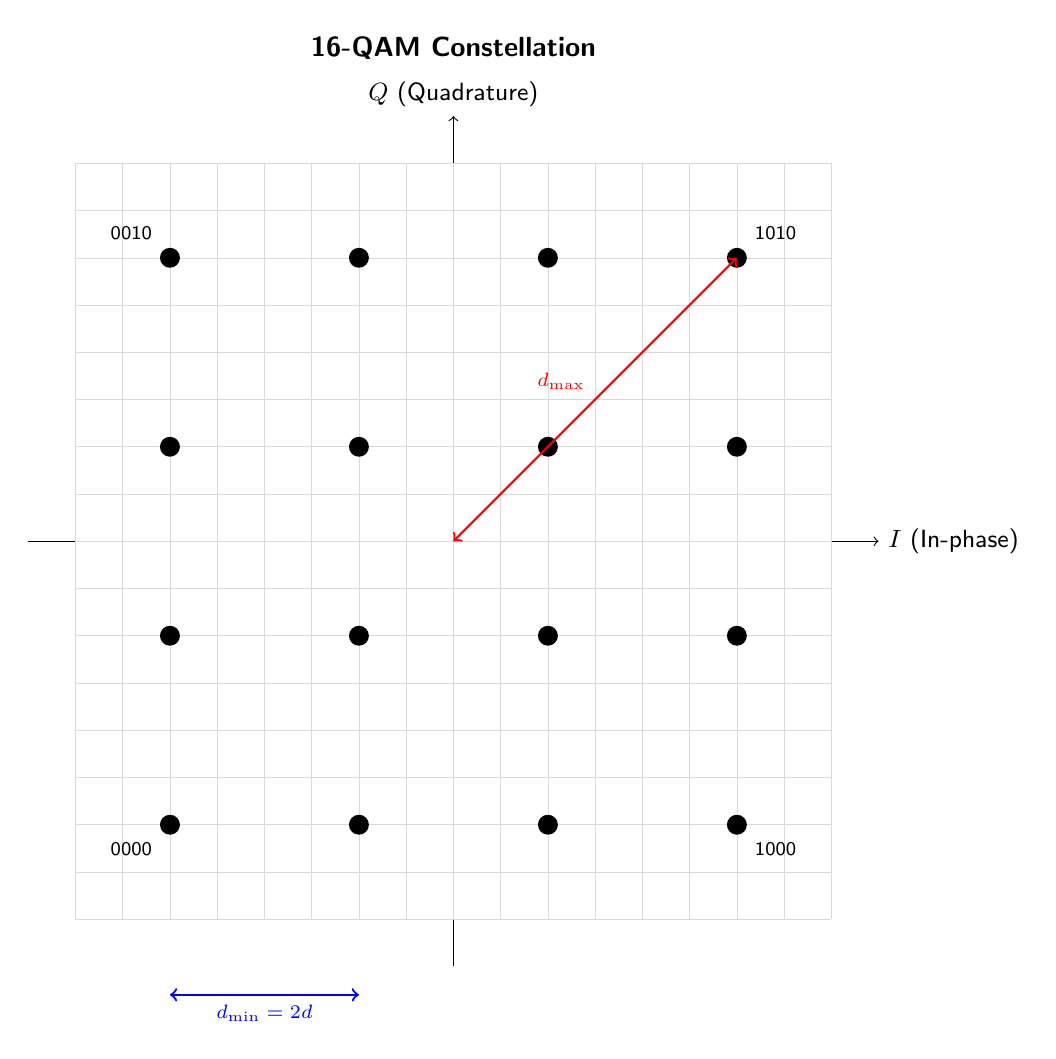
\begin{tikzpicture}[scale=1.2]
% Axes
\draw[->] (-4.5,0) -- (4.5,0) node[right] {\sffamily\small $I$ (In-phase)};
\draw[->] (0,-4.5) -- (0,4.5) node[above] {\sffamily\small $Q$ (Quadrature)};

% Grid
\draw[very thin,gray!30] (-4,-4) grid[step=0.5] (4,4);

% Constellation points (d=1 normalized)
\foreach \i in {-3,-1,1,3} {
  \foreach \q in {-3,-1,1,3} {
    \fill[black] (\i,\q) circle (3pt);
  }
}

% Labels for corner points
\node[below left=3pt] at (-3,-3) {\sffamily\scriptsize 0000};
\node[above left=3pt] at (-3,3) {\sffamily\scriptsize 0010};
\node[above right=3pt] at (3,3) {\sffamily\scriptsize 1010};
\node[below right=3pt] at (3,-3) {\sffamily\scriptsize 1000};

% Distance annotation
\draw[<->,thick,blue] (-3,-4.8) -- (-1,-4.8) node[midway,below,font=\scriptsize] {$d_{\min} = 2d$};
\draw[<->,thick,red] (0,0) -- (3,3) node[midway,above left,font=\scriptsize] {$d_{\max}$};

% Title
\node[above,font=\sffamily\bfseries] at (0,5) {16-QAM Constellation};
\end{tikzpicture}
\end{center}

\textbf{Amplitude levels}: $I, Q \in \{-3d, -d, +d, +3d\}$

where $d$ = unit spacing (normalized distance)

\subsubsection{Bit Mapping (Gray Coding)}\label{bit-mapping-gray-coding}

\textbf{4 bits per symbol}: \(b_3 b_2 b_1 b_0\)

\textbf{Typical mapping}: - \(b_3 b_2\) \$\textbackslash rightarrow\$ I
component (00=-3d, 01=-d, 11=+d, 10=+3d) - \(b_1 b_0\)
\$\textbackslash rightarrow\$ Q component (00=-3d, 01=-d, 11=+d, 10=+3d)

\textbf{Example symbols}:

{\def\LTcaptype{} % do not increment counter
\begin{longtable}[]{@{}llll@{}}
\toprule\noalign{}
Bits & I & Q & Position \\
\midrule\noalign{}
\endhead
\bottomrule\noalign{}
\endlastfoot
0000 & -3d & -3d & Bottom-left corner \\
0001 & -3d & -d & \\
0011 & -3d & +d & \\
0010 & -3d & +3d & Top-left corner \\
1010 & +3d & +3d & Top-right corner \\
\end{longtable}
}

\textbf{Gray coding}: Adjacent symbols differ by exactly 1 bit, minimizing bit errors when symbol errors occur.

\subsubsection{Signal Characteristics}

The average symbol energy for 16-QAM is:
\begin{equation}
\bar{E}_s = \frac{1}{16}\sum_{m=0}^{15} (I_m^2 + Q_m^2) = \frac{1}{16} \times 16 \times 10d^2 = 10d^2
\label{eq:16qam-energy}
\end{equation}

For unit average energy normalization, set $d^2 = 1/10$, giving $\bar{E}_s = 1$.

The minimum Euclidean distance between adjacent constellation points is:
\begin{equation}
d_{\min} = 2d = 2\sqrt{\frac{1}{10}} = \frac{2}{\sqrt{10}} \approx 0.632
\label{eq:16qam-distance}
\end{equation}

\subsection{64-QAM}

\subsubsection{Constellation Diagram}

The 64-QAM constellation forms an $8 \times 8$ square grid:

\begin{center}
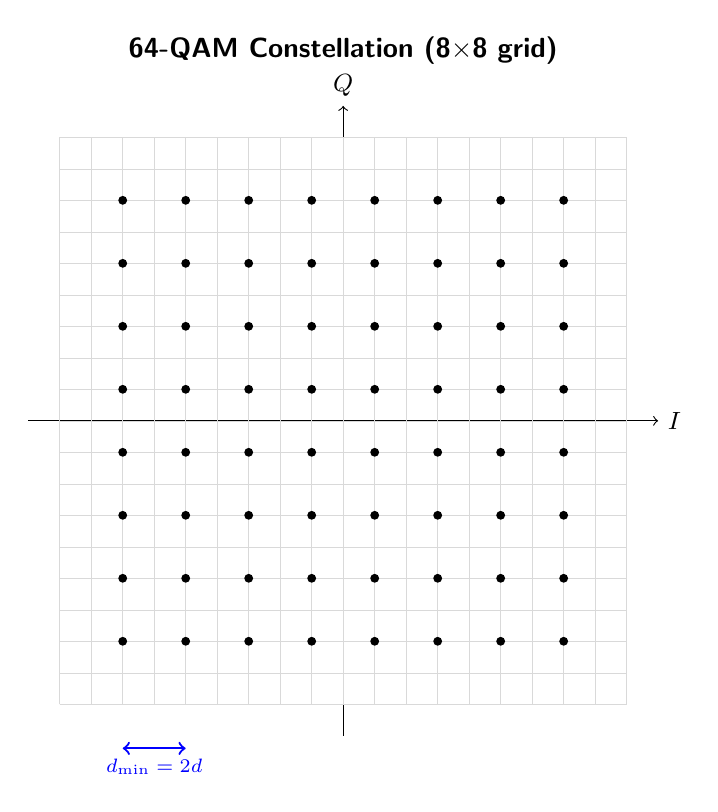
\begin{tikzpicture}[scale=0.8]
% Axes
\draw[->] (-5,0) -- (5,0) node[right] {\sffamily\small $I$};
\draw[->] (0,-5) -- (0,5) node[above] {\sffamily\small $Q$};

% Grid
\draw[very thin,gray!30] (-4.5,-4.5) grid[step=0.5] (4.5,4.5);

% Constellation points (8x8 grid, d=0.5 for spacing)
\foreach \i in {-3.5,-2.5,-1.5,-0.5,0.5,1.5,2.5,3.5} {
  \foreach \q in {-3.5,-2.5,-1.5,-0.5,0.5,1.5,2.5,3.5} {
    \fill[black] (\i,\q) circle (2pt);
  }
}

% Distance annotation
\draw[<->,thick,blue] (-3.5,-5.2) -- (-2.5,-5.2) node[midway,below,font=\scriptsize] {$d_{\min} = 2d$};

% Title
\node[above,font=\sffamily\bfseries] at (0,5.5) {64-QAM Constellation (8$\times$8 grid)};
\end{tikzpicture}
\end{center}

\textbf{Amplitude levels}: $I, Q \in \{-7d, -5d, -3d, -d, +d, +3d, +5d, +7d\}$

\textbf{Bits per symbol}: $k = \log_2(64) = 6$

The average symbol energy is:
\begin{equation}
\bar{E}_s = \frac{1}{64}\sum_{m=0}^{63} (I_m^2 + Q_m^2) = 42d^2
\label{eq:64qam-energy}
\end{equation}

For normalized energy ($\bar{E}_s = 1$): $d = 1/\sqrt{42}$

Minimum distance:
\begin{equation}
d_{\min} = 2d = \frac{2}{\sqrt{42}} \approx 0.309
\label{eq:64qam-distance}
\end{equation}

\subsection{256-QAM}

\subsubsection{Constellation Diagram}

256-QAM uses a $16 \times 16$ square grid with 256 constellation points.

\textbf{Bits per symbol}: $k = \log_2(256) = 8$

The average symbol energy is:
\begin{equation}
\bar{E}_s = 170d^2
\label{eq:256qam-energy}
\end{equation}

For normalized energy: $d = 1/\sqrt{170}$

Minimum distance:
\begin{equation}
d_{\min} = 2d = \frac{2}{\sqrt{170}} \approx 0.153
\label{eq:256qam-distance}
\end{equation}

\subsubsection{High-Order QAM}

\textbf{1024-QAM}: $32 \times 32$ grid, 10 bits/symbol

\textbf{4096-QAM}: $64 \times 64$ grid, 12 bits/symbol

\textbf{Practical limit}: $\sim$4096-QAM (802.11ax WiFi 6, DOCSIS 3.1 cable modems)

\begin{warningbox}
High-order QAM (1024-QAM and above) requires \textbf{exceptional channel conditions}:
\begin{itemize}
\item SNR $>$ 30--40~dB (typically achievable only in controlled environments)
\item Excellent transmitter/receiver linearity (EVM $<$ 1\%)
\item Accurate I/Q balance and phase noise control
\item Short transmission distances or high-quality cables
\end{itemize}
In practice, 1024/4096-QAM are limited to WiFi at very close range or wired systems (cable/DSL).
\end{warningbox}

\section{Performance Analysis}

\subsection{Symbol Error Rate (SER)}

For square M-QAM in an AWGN channel (approximate, high SNR):
\begin{equation}
P_s \approx 4\left(1 - \frac{1}{\sqrt{M}}\right) Q\left(\sqrt{\frac{3}{M-1} \cdot \frac{E_s}{N_0}}\right)
\label{eq:qam-ser}
\end{equation}
where:
\begin{itemize}
\item $Q(x) = \frac{1}{\sqrt{2\pi}} \int_x^\infty e^{-t^2/2} dt$ = Gaussian Q-function
\item $E_s$ = average symbol energy (joules)
\item $N_0$ = noise power spectral density (W/Hz)
\item $M$ = constellation size
\end{itemize}

\subsection{Bit Error Rate (BER)}

With Gray coding (adjacent symbols differ by 1 bit), the approximate BER is:
\begin{equation}
\text{BER} \approx \frac{P_s}{\log_2(M)}
\label{eq:qam-ber-gray}
\end{equation}

Expressed in terms of $E_b/N_0$:
\begin{equation}
\text{BER} \approx \frac{4}{\log_2(M)}\left(1 - \frac{1}{\sqrt{M}}\right) Q\left(\sqrt{\frac{3\log_2(M)}{M-1} \cdot \frac{E_b}{N_0}}\right)
\label{eq:qam-ber-eb}
\end{equation}
where $E_b/N_0 = (E_s/N_0) / \log_2(M)$ is the energy per bit to noise ratio.

\subsubsection{Required Eb/N0 for BER =
10\textbackslash textsuperscript\{-\}\textbackslash textsuperscript\{6\}}\label{required-ebn0-for-ber-10ux2076}

{\def\LTcaptype{} % do not increment counter
\begin{longtable}[]{@{}llll@{}}
\toprule\noalign{}
Modulation & Bits/symbol & Required Eb/N0 (dB) & SNR Penalty vs QPSK \\
\midrule\noalign{}
\endhead
\bottomrule\noalign{}
\endlastfoot
\textbf{QPSK} & 2 & 10.5 & 0 dB (baseline) \\
\textbf{16-QAM} & 4 & 14.5 & +4 dB \\
\textbf{64-QAM} & 6 & 18.5 & +8 dB \\
\textbf{256-QAM} & 8 & 23 & +12.5 dB \\
\textbf{1024-QAM} & 10 & 27.5 & +17 dB \\
\textbf{4096-QAM} & 12 & 32 & +21.5 dB \\
\end{longtable}
}

\textbf{Pattern}: Each 4\$\textbackslash times\$ increase in M adds
\textasciitilde4 dB

\begin{center}\rule{0.5\linewidth}{0.5pt}\end{center}

\subsubsection{BER Comparison Table}\label{ber-comparison-table}

{\def\LTcaptype{} % do not increment counter
\begin{longtable}[]{@{}lllll@{}}
\toprule\noalign{}
Eb/N0 (dB) & QPSK & 16-QAM & 64-QAM & 256-QAM \\
\midrule\noalign{}
\endhead
\bottomrule\noalign{}
\endlastfoot
10 &
3.9\$\textbackslash times\$10\textbackslash textsuperscript\{-\}\textbackslash textsuperscript\{6\}
&
2\$\textbackslash times\$10\textbackslash textsuperscript\{-\}\textbackslash textsuperscript\{3\}
& 0.1 & 0.3 \\
15 &
7\$\textbackslash times\$10\textbackslash textsuperscript\{-\}\textbackslash textsuperscript\{1\}\textbackslash textsuperscript\{0\}
&
5\$\textbackslash times\$10\textbackslash textsuperscript\{-\}\textbackslash textsuperscript\{6\}
&
5\$\textbackslash times\$10\textbackslash textsuperscript\{-\}\textbackslash textsuperscript\{3\}
& 0.08 \\
20 &
\textless10\textbackslash textsuperscript\{-\}\textbackslash textsuperscript\{1\}\textbackslash textsuperscript\{2\}
&
1\$\textbackslash times\$10\textbackslash textsuperscript\{-\}\textbackslash textsuperscript\{9\}
&
1\$\textbackslash times\$10\textbackslash textsuperscript\{-\}\textbackslash textsuperscript\{5\}
&
3\$\textbackslash times\$10\textbackslash textsuperscript\{-\}\textbackslash textsuperscript\{3\} \\
25 &
\textless10\textbackslash textsuperscript\{-\}\textbackslash textsuperscript\{1\}\textbackslash textsuperscript\{2\}
&
\textless10\textbackslash textsuperscript\{-\}\textbackslash textsuperscript\{1\}\textbackslash textsuperscript\{2\}
&
1\$\textbackslash times\$10\textbackslash textsuperscript\{-\}\textbackslash textsuperscript\{8\}
&
2\$\textbackslash times\$10\textbackslash textsuperscript\{-\}\textbackslash textsuperscript\{5\} \\
30 &
\textless10\textbackslash textsuperscript\{-\}\textbackslash textsuperscript\{1\}\textbackslash textsuperscript\{2\}
&
\textless10\textbackslash textsuperscript\{-\}\textbackslash textsuperscript\{1\}\textbackslash textsuperscript\{2\}
&
\textless10\textbackslash textsuperscript\{-\}\textbackslash textsuperscript\{1\}\textbackslash textsuperscript\{2\}
&
2\$\textbackslash times\$10\textbackslash textsuperscript\{-\}\textbackslash textsuperscript\{8\} \\
\end{longtable}
}

\begin{center}\rule{0.5\linewidth}{0.5pt}\end{center}

\section{Bandwidth Efficiency}

With raised-cosine pulse shaping (roll-off factor $\alpha$), the occupied bandwidth is:
\begin{equation}
B = (1 + \alpha) R_s = (1 + \alpha) \frac{R_b}{\log_2(M)} \quad \text{(Hz)}
\label{eq:qam-bandwidth}
\end{equation}
where:
\begin{itemize}
\item $R_b$ = bit rate (bps)
\item $R_s$ = symbol rate (symbols/sec)
\item $\alpha$ = roll-off factor (typically 0.2--0.5)
\end{itemize}

The spectral efficiency is:
\begin{equation}
\eta = \frac{R_b}{B} = \frac{\log_2(M)}{1 + \alpha} \quad \text{(bits/sec/Hz)}
\label{eq:qam-spectral-efficiency}
\end{equation}

\subsubsection{Comparison (\$\textbackslash alpha\$ =
0.35)}\label{comparison-ux3b1-0.35}

{\def\LTcaptype{} % do not increment counter
\begin{longtable}[]{@{}llll@{}}
\toprule\noalign{}
Modulation & Bits/symbol & Spectral Efficiency & Practical Limit \\
\midrule\noalign{}
\endhead
\bottomrule\noalign{}
\endlastfoot
\textbf{QPSK} & 2 & 1.48 & Good SNR (10 dB) \\
\textbf{16-QAM} & 4 & 2.96 & Moderate SNR (15 dB) \\
\textbf{64-QAM} & 6 & 4.44 & High SNR (20 dB) \\
\textbf{256-QAM} & 8 & 5.93 & Very high SNR (25 dB) \\
\textbf{1024-QAM} & 10 & 7.41 & Excellent SNR (30 dB), wired only \\
\textbf{4096-QAM} & 12 & 8.89 & Exceptional SNR (35 dB), cable/DSL \\
\end{longtable}
}

\section{Worked Example: WiFi Link with 64-QAM}

\begin{calloutbox}{Example: 802.11ac Link Budget Analysis}

\textbf{Scenario:} Indoor WiFi link using 64-QAM at 5~GHz

\subsection*{Given Parameters}
\begin{tabular}{@{}ll@{}}
Frequency & $f = 5.2$~GHz (802.11ac) \\
Distance & $d = 10$~m (indoor) \\
TX power & $P_t = 20$~dBm (100~mW) \\
TX antenna gain & $G_t = 2$~dBi (omnidirectional) \\
RX antenna gain & $G_r = 2$~dBi (laptop) \\
Bandwidth & $B = 20$~MHz \\
Modulation & 64-QAM (6 bits/symbol) \\
Coding rate & $r = 3/4$ \\
Noise figure & $NF = 6$~dB \\
Target BER & $10^{-6}$ \\
\end{tabular}

\subsection*{Step 1: Free-Space Path Loss}
\begin{equation*}
\mathrm{FSPL} = 20\log_{10}(d) + 20\log_{10}(f) + 32.45 = 20\log_{10}(10) + 20\log_{10}(5200) + 32.45
\end{equation*}
\begin{equation*}
\mathrm{FSPL} = 20 + 74.3 + 32.45 = 126.8~\text{dB}
\end{equation*}

\subsection*{Step 2: Indoor Propagation Loss}
Indoor walls and obstacles add approximately 15~dB additional loss:
\begin{equation*}
L_{\text{indoor}} = 15~\text{dB}
\end{equation*}

\subsection*{Step 3: Received Signal Power}
\begin{equation*}
P_r = P_t + G_t + G_r - \mathrm{FSPL} - L_{\text{indoor}}
\end{equation*}
\begin{equation*}
P_r = 20 + 2 + 2 - 126.8 - 15 = -117.8~\text{dBm}
\end{equation*}

\subsection*{Step 4: Noise Power}
\begin{equation*}
N = kTB \cdot NF = (-174 + 10\log_{10}(20 \times 10^6) + 6)~\text{dBm}
\end{equation*}
\begin{equation*}
N = -174 + 73 + 6 = -95~\text{dBm}
\end{equation*}

\subsection*{Step 5: Signal-to-Noise Ratio}
\begin{equation*}
\mathrm{SNR} = P_r - N = -117.8 - (-95) = -22.8~\text{dB} \quad \text{(Oops! Negative!)}
\end{equation*}

Wait, this link won't work! Let's recalculate with a more realistic scenario at $d = 5$~m:
\begin{equation*}
\mathrm{FSPL}(5~\text{m}) = 20 + 68.3 + 32.45 = 120.8~\text{dB}
\end{equation*}
\begin{equation*}
P_r = 20 + 2 + 2 - 120.8 - 10 = -106.8~\text{dBm}
\end{equation*}
\begin{equation*}
\mathrm{SNR} = -106.8 - (-95) = -11.8~\text{dB} \quad \text{(Still negative!)}
\end{equation*}

\textbf{Actually}, the symbol rate for 20~MHz 802.11ac is $R_s \approx 312.5$~kSymbols/sec (accounting for OFDM overhead), so effective bandwidth is narrower. Using $B_{\text{eff}} = 16.25$~MHz:
\begin{equation*}
N = -174 + 72.1 + 6 = -95.9~\text{dBm}
\end{equation*}
\begin{equation*}
\mathrm{SNR} = -106.8 - (-95.9) = -10.9~\text{dB} \quad \text{(Still too low!)}
\end{equation*}

\textbf{Correct approach - use symbol rate:}
\begin{equation*}
R_b = 6~\text{bits/symbol} \times \frac{3}{4}~\text{(coding)} \times 312.5~\text{kSymbols/sec} \approx 1.4~\text{Mbps per subcarrier}
\end{equation*}

For 52 data subcarriers (802.11ac), total rate $\approx 73$~Mbps.

\subsection*{Step 6: Required $E_b/N_0$ for 64-QAM}
From equation~\ref{eq:qam-ber-eb}, for BER $= 10^{-6}$ with 64-QAM: $E_b/N_0 \approx 18.5$~dB

\subsection*{Conclusion}
The link margin is tight. In practice, 802.11ac would use adaptive modulation:
\begin{itemize}
\item \textbf{Close range (< 5~m)}: 256-QAM possible
\item \textbf{Medium range (5--15~m)}: 64-QAM typical
\item \textbf{Long range (> 20~m)}: Falls back to 16-QAM or QPSK
\end{itemize}

\textbf{Key insight:} This calculation shows why WiFi speed drops dramatically with distance---the system must switch to lower-order QAM to maintain link reliability.
\end{calloutbox}

\section{Modulation and Demodulation}

\subsection{QAM Modulator}

The QAM modulator uses standard I/Q (quadrature) modulation architecture:

\begin{center}
\begin{tikzpicture}[
  block/.style={rectangle, draw, minimum width=2cm, minimum height=1cm, font=\sffamily\small},
  sum/.style={circle, draw, minimum size=0.8cm, font=\sffamily\small},
  node distance=2.2cm,
  font=\small
]
% Input
\node (input) {\sffamily Serial\\Data};
\node[block, right of=input, node distance=2.5cm] (serial) {Serial to\\Parallel};

% I branch
\node[block, above right of=serial, node distance=3cm] (imap) {I-Symbol\\Mapper};
\node[block, right of=imap, node distance=3cm] (imult) {Mixer\\$\times$};
\node[above of=imult, node distance=1.3cm, font=\scriptsize] (cos) {$\cos(2\pi f_c t)$};

% Q branch
\node[block, below right of=serial, node distance=3cm] (qmap) {Q-Symbol\\Mapper};
\node[block, right of=qmap, node distance=3cm] (qmult) {Mixer\\$\times$};
\node[below of=qmult, node distance=1.3cm, font=\scriptsize] (sin) {$-\sin(2\pi f_c t)$};

% Summer
\node[sum, right of=imult, node distance=2.5cm, yshift=-1.5cm] (sum) {$+$};

% Output
\node[block, right of=sum, node distance=2.5cm] (filter) {Bandpass\\Filter};
\node[right of=filter, node distance=2.5cm] (output) {\sffamily QAM\\Output};

% Connections
\draw[->,thick] (input) -- (serial);
\draw[->,thick] (serial) |- (imap);
\draw[->,thick] (serial) |- (qmap);
\draw[->,thick] (imap) -- node[above,font=\scriptsize] {$I(t)$} (imult);
\draw[->,thick] (qmap) -- node[above,font=\scriptsize] {$Q(t)$} (qmult);
\draw[->,thick] (cos) -- (imult);
\draw[->,thick] (sin) -- (qmult);
\draw[->,thick] (imult) -- (sum);
\draw[->,thick] (qmult) -- (sum);
\draw[->,thick] (sum) -- (filter);
\draw[->,thick] (filter) -- (output);
\end{tikzpicture}
\end{center}

\textbf{Note:} The hardware is identical to QPSK; only the symbol mapping differs (QAM uses multiple amplitude levels).

\subsection{QAM Coherent Demodulator}

The receiver uses coherent I/Q demodulation to recover the transmitted symbols:

\begin{center}
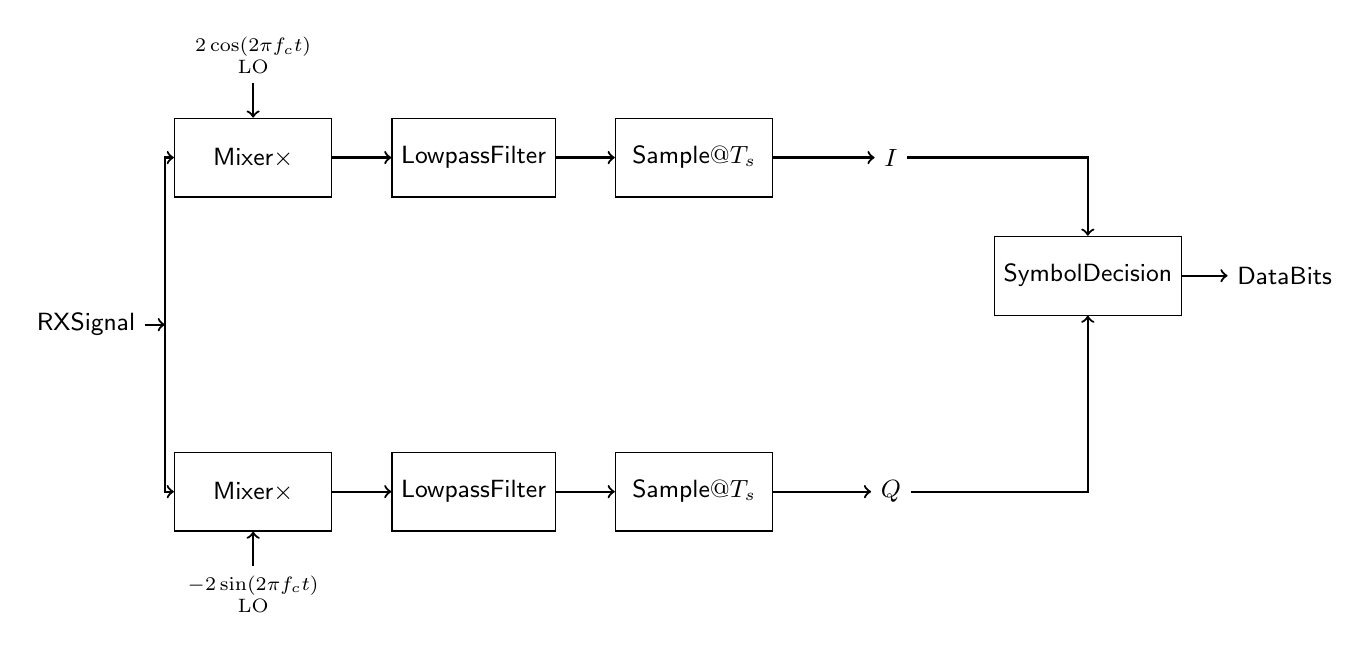
\begin{tikzpicture}[
  block/.style={rectangle, draw, minimum width=2cm, minimum height=1cm, font=\sffamily\small},
  node distance=2.2cm,
  font=\small
]
% Input
\node (input) {\sffamily RX\\Signal};

% I branch
\node[block, above right of=input, node distance=3cm] (imult) {Mixer\\$\times$};
\node[above of=imult, node distance=1.3cm, font=\scriptsize, align=center] (cos) {$2\cos(2\pi f_c t)$\\LO};
\node[block, right of=imult, node distance=2.8cm] (ilpf) {Lowpass\\Filter};
\node[block, right of=ilpf, node distance=2.8cm] (isample) {Sample\\$@T_s$};
\node[right of=isample, node distance=2.5cm] (iout) {\sffamily $I$};

% Q branch  
\node[block, below right of=input, node distance=3cm] (qmult) {Mixer\\$\times$};
\node[below of=qmult, node distance=1.3cm, font=\scriptsize, align=center] (sin) {$-2\sin(2\pi f_c t)$\\LO};
\node[block, right of=qmult, node distance=2.8cm] (qlpf) {Lowpass\\Filter};
\node[block, right of=qlpf, node distance=2.8cm] (qsample) {Sample\\$@T_s$};
\node[right of=qsample, node distance=2.5cm] (qout) {\sffamily $Q$};

% Decision block
\node[block, right of=isample, node distance=5cm, yshift=-1.5cm] (decision) {Symbol\\Decision};
\node[right of=decision, node distance=2.5cm] (bits) {\sffamily Data\\Bits};

% Connections
\draw[->,thick] (input) -- ++(1,0) coordinate(split);
\draw[->,thick] (split) |- (imult);
\draw[->,thick] (split) |- (qmult);
\draw[->,thick] (cos) -- (imult);
\draw[->,thick] (sin) -- (qmult);
\draw[->,thick] (imult) -- (ilpf);
\draw[->,thick] (ilpf) -- (isample);
\draw[->,thick] (isample) -- (iout);
\draw[->,thick] (qmult) -- (qlpf);
\draw[->,thick] (qlpf) -- (qsample);
\draw[->,thick] (qsample) -- (qout);
\draw[->,thick] (iout) -| (decision);
\draw[->,thick] (qout) -| (decision);
\draw[->,thick] (decision) -- (bits);
\end{tikzpicture}
\end{center}

\textbf{Detection process:}
\begin{enumerate}
\item Sample I and Q at symbol rate $T_s$
\item Find nearest constellation point (minimum Euclidean distance)
\item Map constellation point to bits using Gray code mapping
\end{enumerate}

\subsubsection{Soft-Decision Decoding}\label{soft-decision-decoding}

\textbf{Hard decision}: Nearest neighbor \$\textbackslash rightarrow\$
Bits

\textbf{Soft decision}: Pass I/Q values (or LLRs) to decoder

\textbf{Log-Likelihood Ratio (LLR)} for bit \(b_k\):

\[
\text{LLR}(b_k) = \log\frac{P(b_k=0 | r)}{P(b_k=1 | r)}
\]

\textbf{Benefit}: \textasciitilde2 dB coding gain (LDPC, Turbo codes use
soft decisions)

\begin{center}\rule{0.5\linewidth}{0.5pt}\end{center}

\subsection{Power Efficiency}\label{power-efficiency}

\subsubsection{Peak-to-Average Power Ratio
(PAPR)}\label{peak-to-average-power-ratio-papr}

\textbf{QAM has varying envelope}:

\[
|s_m| = \sqrt{I_m^2 + Q_m^2}
\]

\textbf{PAPR}:

\[
\text{PAPR} = \frac{P_{\max}}{P_{\text{avg}}} = \frac{|s_{\max}|^2}{\bar{E}_s}
\]

\begin{center}\rule{0.5\linewidth}{0.5pt}\end{center}

\subsubsection{PAPR Values}\label{papr-values}

{\def\LTcaptype{} % do not increment counter
\begin{longtable}[]{@{}llll@{}}
\toprule\noalign{}
Modulation & PAPR (linear) & PAPR (dB) & Notes \\
\midrule\noalign{}
\endhead
\bottomrule\noalign{}
\endlastfoot
\textbf{QPSK} & 1 & 0 dB & Constant envelope \\
\textbf{16-QAM} & 2.55 & 4.1 dB & Corner points
2.55\$\textbackslash times\$ average \\
\textbf{64-QAM} & 3.68 & 5.7 dB & \\
\textbf{256-QAM} & 4.80 & 6.8 dB & \\
\textbf{1024-QAM} & 5.93 & 7.7 dB & \\
\end{longtable}
}

\textbf{Impact}: High PAPR requires PA backoff (reduces efficiency)

\textbf{Example}: 64-QAM with 5.7 dB PAPR - PA must back off 5.7 dB from
saturation - Efficiency drops from 50\% to \textasciitilde13\%
(4\$\textbackslash times\$ penalty)

\begin{center}\rule{0.5\linewidth}{0.5pt}\end{center}

\subsection{Practical Impairments}\label{practical-impairments}

\subsubsection{1. I/Q Imbalance}\label{iq-imbalance}

\textbf{Gain mismatch}: \(G_I \neq G_Q\)

\textbf{Phase error}: 90\$\^{}\textbackslash circ\$ hybrid imperfect
(e.g., 88\$\^{}\textbackslash circ\$ or 92\$\^{}\textbackslash circ\$)

\textbf{Effect}: Constellation distortion, image leakage

\textbf{Model}:

\[
r = (1 + \alpha_G) I + j(1 - \alpha_G) e^{j\epsilon} Q + n
\]

Where: - \(\alpha_G\) = Gain imbalance - \(\epsilon\) = Phase error

\textbf{Typical}: \$\textbackslash pm\$0.5 dB gain,
\$\textbackslash pm\$2\$\^{}\textbackslash circ\$ phase (degrades
256-QAM significantly)

\textbf{Mitigation}: Digital calibration (pilot-aided estimation)

\begin{center}\rule{0.5\linewidth}{0.5pt}\end{center}

\subsubsection{2. Nonlinear PA
Distortion}\label{nonlinear-pa-distortion}

\textbf{AM-AM conversion}: Gain compression at high amplitudes

\textbf{AM-PM conversion}: Phase shift varies with amplitude

\textbf{Effect}: Constellation warping, especially outer points

\textbf{Example}: 64-QAM, corner points compress 1 dB - Minimum distance
reduced \$\textbackslash rightarrow\$ BER increases - Spectral regrowth
(adjacent channel interference)

\textbf{Mitigation}: - \textbf{Backoff}: 6-10 dB (kills efficiency) -
\textbf{Predistortion}: Digital (DPD) or analog - \textbf{Crest factor
reduction (CFR)}: Clip peaks, re-generate signal

\begin{center}\rule{0.5\linewidth}{0.5pt}\end{center}

\subsubsection{3. Phase Noise}\label{phase-noise}

\textbf{Oscillator jitter} causes constellation rotation/spread:

\[
r(t) = s(t) e^{j\phi_n(t)} + n(t)
\]

\textbf{Effect}: Common phase error (CPE) + inter-carrier interference
(OFDM)

\textbf{Sensitivity}: Higher-order QAM more sensitive

\textbf{Example}: 256-QAM - Tolerable phase noise:
\textasciitilde1\$\^{}\textbackslash circ\$ RMS - Requires high-quality
oscillator (PLL, TCXO, or OCXO)

\begin{center}\rule{0.5\linewidth}{0.5pt}\end{center}

\subsubsection{4. Timing Jitter}\label{timing-jitter}

\textbf{Symbol clock error} causes sampling offset:

\textbf{Effect}: ISI, constellation blurring

\textbf{Requirement}: Timing error \textless{} 0.1 symbol period

\textbf{Example}: 64-QAM @ 10 Msps - Symbol period: 100 ns - Tolerable
jitter: \textless{} 10 ns RMS

\begin{center}\rule{0.5\linewidth}{0.5pt}\end{center}

\subsection{Practical Applications}\label{practical-applications}

\subsubsection{1. WiFi (802.11a/n/ac/ax)}\label{wifi-802.11anacax}

\textbf{OFDM subcarriers} use QAM:

{\def\LTcaptype{} % do not increment counter
\begin{longtable}[]{@{}llll@{}}
\toprule\noalign{}
Standard & Max QAM & Max Rate & Notes \\
\midrule\noalign{}
\endhead
\bottomrule\noalign{}
\endlastfoot
\textbf{802.11a} & 64-QAM & 54 Mbps & 20 MHz channel \\
\textbf{802.11n} & 64-QAM & 600 Mbps & 4\$\textbackslash times\$4 MIMO,
40 MHz \\
\textbf{802.11ac} & 256-QAM & 6.9 Gbps & 8\$\textbackslash times\$8
MIMO, 160 MHz \\
\textbf{802.11ax} (WiFi 6) & 1024-QAM & 9.6 Gbps & OFDMA, MU-MIMO \\
\end{longtable}
}

\textbf{Adaptive modulation}: Switch QPSK \$\textbackslash rightarrow\$
16/64/256/1024-QAM based on SNR

\begin{center}\rule{0.5\linewidth}{0.5pt}\end{center}

\subsubsection{2. LTE/5G NR}\label{lte5g-nr}

\textbf{LTE downlink}: Up to 256-QAM (Cat 9+)

\textbf{5G NR}: Up to 256-QAM (mmWave can use 1024-QAM in some
scenarios)

\textbf{Example}: LTE Cat 16 (1 Gbps downlink) -
4\$\textbackslash times\$4 MIMO, 256-QAM, 20 MHz carrier aggregation -
Per-carrier: 4 layers \$\textbackslash times\$ 8 bits/symbol
\$\textbackslash times\$ 75k symbols/sec = 2.4 Gbps (theoretical)

\textbf{Adaptive MCS} (Modulation \& Coding Scheme): - Poor channel:
QPSK 1/4 (0.5 bits/symbol effective) - Good channel: 256-QAM 3/4 (6
bits/symbol effective)

\begin{center}\rule{0.5\linewidth}{0.5pt}\end{center}

\subsubsection{3. Cable Modems (DOCSIS)}\label{cable-modems-docsis}

\textbf{DOCSIS 3.0}: 256-QAM (8 bits/symbol)

\textbf{DOCSIS 3.1}: 4096-QAM (12 bits/symbol) - Requires SNR
\textgreater{} 40 dB (excellent cable plant) - OFDM with 4096-QAM
subcarriers \$\textbackslash rightarrow\$ 10 Gbps downstream

\textbf{Key}: Wired channel (no fading), high SNR possible

\begin{center}\rule{0.5\linewidth}{0.5pt}\end{center}

\subsubsection{4. Digital TV}\label{digital-tv}

\textbf{DVB-C (Cable)}: 256-QAM standard

\textbf{DVB-T2 (Terrestrial)}: Up to 256-QAM (typically 64-QAM)

\textbf{ATSC 3.0 (US)}: 256-QAM, 1024-QAM, 4096-QAM (OFDM)

\begin{center}\rule{0.5\linewidth}{0.5pt}\end{center}

\subsubsection{5. Microwave Backhaul}\label{microwave-backhaul}

\textbf{Point-to-point links}: - \textbf{Clear weather}: 2048-QAM,
4096-QAM (\$\textbackslash geq\$30 dB SNR) - \textbf{Light rain}:
256-QAM - \textbf{Heavy rain}: Adaptive down to 16-QAM or QPSK

\textbf{Frequency}: 6-42 GHz (E-band: 70-80 GHz)

\textbf{Example}: 28 GHz link, 56 MHz channel - 4096-QAM: 12 bits/symbol
\$\textbackslash rightarrow\$ 672 Mbps (no coding) - With FEC 3/4: 504
Mbps net

\begin{center}\rule{0.5\linewidth}{0.5pt}\end{center}

\subsection{QAM vs PSK}\label{qam-vs-psk}

\textbf{Same spectral efficiency}:

{\def\LTcaptype{} % do not increment counter
\begin{longtable}[]{@{}lll@{}}
\toprule\noalign{}
M-PSK & M-QAM & Comparison \\
\midrule\noalign{}
\endhead
\bottomrule\noalign{}
\endlastfoot
4-PSK (QPSK) & 4-QAM (identical) & Same constellation \\
8-PSK & 8-QAM (rare) & 8-PSK used (const envelope) \\
16-PSK & 16-QAM & \textbf{16-QAM 4 dB better} \\
32-PSK & 32-QAM & \textbf{32-QAM much better} \\
64-PSK & 64-QAM & \textbf{64-QAM far superior} \\
\end{longtable}
}

\textbf{General rule}: For M \textgreater{} 8, QAM always better than
M-PSK

\textbf{Reason}: 2D rectangular grid (QAM) uses signal space more
efficiently than circle (PSK)

\begin{center}\rule{0.5\linewidth}{0.5pt}\end{center}

\subsection{Non-Square QAM}\label{non-square-qam}

\textbf{Cross QAM}: Non-square constellations (e.g., 32-QAM, 128-QAM)

\textbf{32-QAM}: 5 bits/symbol - Constellation: 4 inner points + 12
middle + 16 outer (hexagonal-like) - Used in some proprietary systems

\textbf{128-QAM}: 7 bits/symbol - Between 64-QAM and 256-QAM

\textbf{Trade-off}: Slightly worse performance than square QAM, but
allows finer granularity

\begin{center}\rule{0.5\linewidth}{0.5pt}\end{center}

\subsection{Constellation Shaping}\label{constellation-shaping}

\textbf{Probabilistic shaping}: Non-uniform symbol probability

\textbf{Idea}: Transmit inner points more often (lower energy)
\$\textbackslash rightarrow\$ Reduce average power

\textbf{Benefit}: \textasciitilde0.5-1 dB SNR gain (approaching Shannon
limit)

\textbf{Used in}: Optical communications (400G/800G), submarine cables

\begin{center}\rule{0.5\linewidth}{0.5pt}\end{center}

\subsection{Adaptive QAM}\label{adaptive-qam}

\textbf{Link adaptation}: Select QAM order based on channel

\textbf{SNR thresholds} (example):

{\def\LTcaptype{} % do not increment counter
\begin{longtable}[]{@{}llll@{}}
\toprule\noalign{}
SNR (dB) & Modulation & Code Rate & Spectral Eff. \\
\midrule\noalign{}
\endhead
\bottomrule\noalign{}
\endlastfoot
0-5 & QPSK & 1/2 & 1.0 \\
5-10 & QPSK & 3/4 & 1.5 \\
10-15 & 16-QAM & 1/2 & 2.0 \\
15-20 & 16-QAM & 3/4 & 3.0 \\
20-25 & 64-QAM & 2/3 & 4.0 \\
25-30 & 64-QAM & 3/4 & 4.5 \\
30-35 & 256-QAM & 3/4 & 6.0 \\
\textgreater35 & 1024-QAM & 5/6 & 8.3 \\
\end{longtable}
}

\textbf{Used in}: All modern wireless (WiFi, LTE, 5G)

\section{Advantages and Disadvantages}

\subsection*{Advantages}

\begin{enumerate}
\item \textbf{Superior spectral efficiency:} QAM achieves the highest bits/sec/Hz for a given constellation size compared to PSK or ASK alone.

\item \textbf{Flexible data rates:} Support for multiple QAM orders (16, 64, 256, 1024-QAM) enables adaptive modulation to match channel conditions.

\item \textbf{Optimal signal space utilization:} Rectangular grid constellation uses 2D I/Q space more efficiently than phase-only modulation (PSK).

\item \textbf{Standard implementation:} Same I/Q hardware as QPSK; only symbol mapping differs. Compatible with standard RF architectures.

\item \textbf{Well-suited for OFDM:} Each subcarrier can use independent QAM order, enabling fine-grained rate adaptation.
\end{enumerate}

\subsection*{Disadvantages}

\begin{enumerate}
\item \textbf{High SNR requirement:} Higher-order QAM (256-QAM and above) requires excellent channel conditions (SNR $>$ 25~dB).

\item \textbf{Non-constant envelope:} Variable amplitude increases PAPR (Peak-to-Average Power Ratio), requiring linear amplifiers with reduced efficiency.

\item \textbf{Sensitive to impairments:} Susceptible to:
  \begin{itemize}
  \item I/Q imbalance (gain/phase mismatch between branches)
  \item Phase noise (degrades SNR, especially for high-order QAM)
  \item Nonlinear distortion (amplifier compression)
  \item Frequency/timing offsets
  \end{itemize}

\item \textbf{Coherent detection required:} Receiver must maintain accurate carrier phase and frequency synchronization.

\item \textbf{Performance degradation in fading:} Rapid channel variations (mobility, multipath) force fallback to lower-order QAM, reducing throughput.

\item \textbf{Higher complexity:} Symbol decision requires 2D nearest-neighbor search (vs 1D threshold for BPSK/OOK).
\end{enumerate}

\subsection{Implementation Tips}

\subsubsection{Constellation
Normalization}\label{constellation-normalization}

\textbf{Normalize average power to 1}:

\[
\bar{E}_s = \frac{1}{M}\sum_{m=0}^{M-1} |s_m|^2 = 1
\]

\textbf{Example (16-QAM)}: - Un-normalized:
\(I, Q \in \{-3, -1, +1, +3\}\) - Average power: 10 - Normalized:
\(I, Q \in \{-3, -1, +1, +3\}/\sqrt{10}\)

\begin{center}\rule{0.5\linewidth}{0.5pt}\end{center}

\subsubsection{Gray Coding}\label{gray-coding}

\textbf{Map bits \$\textbackslash rightarrow\$ I/Q using Gray code}:

\begin{Shaded}
\begin{Highlighting}[]
\KeywordTok{def}\NormalTok{ qam\_gray\_mapping(bits):}
    \CommentTok{\# 16{-}QAM Gray mapping}
\NormalTok{    gray\_map }\OperatorTok{=}\NormalTok{ [}\BaseNTok{0b00}\NormalTok{, }\BaseNTok{0b01}\NormalTok{, }\BaseNTok{0b11}\NormalTok{, }\BaseNTok{0b10}\NormalTok{]  }\CommentTok{\# Gray sequence}
\NormalTok{    i\_bits }\OperatorTok{=}\NormalTok{ bits[}\DecValTok{0}\NormalTok{:}\DecValTok{2}\NormalTok{]}
\NormalTok{    q\_bits }\OperatorTok{=}\NormalTok{ bits[}\DecValTok{2}\NormalTok{:}\DecValTok{4}\NormalTok{]}
    
\NormalTok{    i\_index }\OperatorTok{=}\NormalTok{ gray\_map.index(i\_bits)}
\NormalTok{    q\_index }\OperatorTok{=}\NormalTok{ gray\_map.index(q\_bits)}
    
\NormalTok{    I }\OperatorTok{=} \DecValTok{2}\OperatorTok{*}\NormalTok{i\_index }\OperatorTok{{-}} \DecValTok{3}  \CommentTok{\# Map to \{{-}3, {-}1, +1, +3\}}
\NormalTok{    Q }\OperatorTok{=} \DecValTok{2}\OperatorTok{*}\NormalTok{q\_index }\OperatorTok{{-}} \DecValTok{3}
    
    \ControlFlowTok{return}\NormalTok{ I }\OperatorTok{+} \OtherTok{1j}\OperatorTok{*}\NormalTok{Q}
\end{Highlighting}
\end{Shaded}

\begin{center}\rule{0.5\linewidth}{0.5pt}\end{center}

\subsubsection{Soft-Decision LLR
Calculation}\label{soft-decision-llr-calculation}

\textbf{For bit \(b_k\) in constellation}:

\[
\text{LLR}(b_k) = \log\frac{\sum_{s \in S_0} e^{-|r-s|^2/(2\sigma^2)}}{\sum_{s \in S_1} e^{-|r-s|^2/(2\sigma^2)}}
\]

Where: - \(S_0\) = Constellation points with \(b_k = 0\) - \(S_1\) =
Constellation points with \(b_k = 1\) - \(r\) = Received symbol -
\(\sigma^2\) = Noise variance

\begin{center}\rule{0.5\linewidth}{0.5pt}\end{center}

\section{Summary}

\begin{center}
\begin{tabular}{@{}ll@{}}
\toprule
\textbf{Parameter} & \textbf{Value/Description} \\
\midrule
Basic principle & Modulate both amplitude \emph{and} phase \\
Constellation & Rectangular grid in I/Q plane \\
Common orders & 16-QAM (4 bits), 64-QAM (6 bits), 256-QAM (8 bits) \\
Spectral efficiency & $\eta = \log_2(M)/(1+\alpha)$ bps/Hz \\
Gray coding & Adjacent symbols differ by 1 bit \\
BER (64-QAM @ 10$^{-6}$) & Requires $E_b/N_0 \approx 18.5$~dB \\
Detection & Coherent I/Q demodulation, nearest neighbor \\
PAPR & Increases with QAM order (non-constant envelope) \\
Key advantage & Optimal use of 2D signal space \\
Key disadvantage & Requires high SNR, sensitive to impairments \\
Primary applications & WiFi, LTE/5G, cable modems, microwave links \\
Adaptive modulation & Switch QAM order based on channel SNR \\
\bottomrule
\end{tabular}
\end{center}

\textbf{Key insight:} QAM achieves the highest spectral efficiency among single-carrier modulation schemes by utilizing both I and Q dimensions. While PSK varies only phase (constant radius) and ASK varies only amplitude (fixed phase), QAM combines both for optimal signal space packing. The trade-off is increased sensitivity to noise and hardware impairments, requiring careful system design and adaptive rate control.

\textbf{Performance comparison:}

\begin{center}
\begin{tabular}{@{}lcccc@{}}
\toprule
\textbf{QAM Order} & \textbf{Bits/Symbol} & \textbf{$d_{\min}$} & \textbf{$E_b/N_0$ @ BER=$10^{-6}$} & \textbf{Typical Use} \\
\midrule
4-QAM (QPSK) & 2 & 1.41 & 10.5~dB & Satellite, long-range \\
16-QAM & 4 & 0.63 & 14.5~dB & WiFi, LTE baseline \\
64-QAM & 6 & 0.31 & 18.5~dB & WiFi, LTE good SNR \\
256-QAM & 8 & 0.15 & 23~dB & WiFi 5/6, LTE-A \\
1024-QAM & 10 & 0.098 & 27.5~dB & WiFi 6 (short range) \\
4096-QAM & 12 & 0.049 & 32~dB & Cable/DSL only \\
\bottomrule
\end{tabular}
\end{center}

\section{Further Reading}

\begin{itemize}
\item \textbf{Chapter~\ref{ch:qpsk}:} QPSK Modulation---the simplest QAM (4-QAM), foundation for understanding QAM
\item \textbf{Chapter~\ref{ch:constellation}:} Constellation Diagrams---visualization and interpretation of QAM signals
\item \textbf{Chapter~\ref{ch:iq}:} IQ Representation---mathematical foundation of quadrature modulation
\item \textbf{Chapter~\ref{ch:ber}:} Bit Error Rate Analysis---performance metrics and measurement
\item \textbf{Chapter~\ref{ch:ofdm}:} OFDM \& Multicarrier---uses QAM on each subcarrier for WiFi/LTE
\item \textbf{Chapter~\ref{ch:adaptive}:} Adaptive Modulation \& Coding---dynamic QAM order selection
\item \textbf{Chapter~\ref{ch:synchronization}:} Carrier/Timing Synchronization---critical for coherent QAM detection
\item \textbf{Chapter~\ref{ch:fec}:} Forward Error Correction---essential for reliable high-order QAM
\item \textbf{Chapter~\ref{ch:channel-models}:} Channel Models---understand fading effects on QAM performance
\item \textbf{Chapter~\ref{ch:ask}:} Amplitude Shift Keying---amplitude-only modulation component
\item \textbf{Chapter~\ref{ch:psk}:} Phase Shift Keying---phase-only modulation component
\item \textbf{Chapter~\ref{ch:shannon}:} Shannon's Channel Capacity---theoretical limits of spectral efficiency
\end{itemize}
